\documentclass{cornouaille}
\begin{document}
\QCMautoevaluation{Pour chaque question, plusieurs réponses sont
  proposées.  Déterminer celles qui sont correctes.}

\begin{QCM}
  \begin{EnonceCommunQCM}
    On considère le cube $ABCDEFGH$ de côté $a$, avec $I$, $J$ les
    milieux respectifs des segments $[CD]$ et $[GH]$ et $L$ est le
    milieu du segment $[GH]$.

    \begin{center}
     \includestandalone{\standalonepath/cubeqcm}
    \end{center}
  \end{EnonceCommunQCM}
  
\begin{GroupeQCM}
  \begin{exercice}
    La droite $(BI)$ est :
    \begin{ChoixQCM}{3}
    \item orthogonale à $(IJ)$
    \item orthogonale à $(IL)$
    \item orthogonale à $(DG)$
    \end{ChoixQCM}
\begin{solution}
      \reponseQCM{a}
\end{solution}
  \end{exercice}

  \begin{exercice}
    L'intersection du plan $(BIL)$ avec le plan $(ABF)$ est :
    \begin{ChoixQCM}{3}
    \item une droite passant par\\ le milieu de $[AB]$
    \item une droite passant par\\ le point $B$
    \item une droite parallèle à $(IL)$
    \end{ChoixQCM}
  \end{exercice}
\begin{solution}
    \reponseQCM{b} et \reponseQCM{c}
\end{solution}

  \begin{exercice}
    La section du cube $ABCDEFGH$ par le plan $(BIL)$ est :
    \begin{ChoixQCM}{3}
    \item un triangle
    \item un parallélogramme
    \item un trapèze
    \end{ChoixQCM}
  \end{exercice}
\begin{solution}
    \reponseQCM{c}
\end{solution}

  \begin{exercice}
    Dans le repère
    $(A;\overrightarrow{AB},\overrightarrow{AD},\overrightarrow{AE})$
    on a :
    \begin{ChoixQCM}{3}
    \item $\overrightarrow{BJ}\begin{pmatrix}
        -0,5\\
        1\\
        1
      \end{pmatrix}$
    \item les points $L$, $I$, $B$ et $F$ sont\\ coplanaires
    \item
      $\overrightarrow{AJ}=2\overrightarrow{AF}+\overrightarrow{GH}-\overrightarrow{CG}$
    \end{ChoixQCM}
  \end{exercice}
\begin{solution}
    \reponseQCM{a}
\end{solution}
\end{GroupeQCM}
\end{QCM}

\begin{QCM}
\begin{EnonceCommunQCM}
  Dans un repère
  $(O\,;\overrightarrow{i},\overrightarrow{j},\overrightarrow{k})$ de
  l'espace, on considère les points $A(1\,;0\,;2)$, $B(2\,;1\,;2)$,
  $C(3\,;0\,;0)$ et $D(5\,;-2\,;-4)$.
\end{EnonceCommunQCM}

\begin{GroupeQCM}
  \begin{exercice}
    Les points $A$, $B$ et $C$ :
    \begin{ChoixQCM}{3}
    \item sont alignés
    \item sont coplanaires
    \item définissent un plan
    \end{ChoixQCM}
  \end{exercice}
\begin{solution}
    \reponseQCM{b} et \reponseQCM{c}
\end{solution}

  \begin{exercice}
    Les points $A$, $B$, $C$ et $D$ :
    \begin{ChoixQCM}{3}
    \item sont coplanaires
    \item vérifient l'égalité\\
      $\overrightarrow{AD}=-2\overrightarrow{AB}+3\overrightarrow{AC}$
    \item $D\in(BC)$
    \end{ChoixQCM}
  \end{exercice}
\begin{solution}
    \reponseQCM{a b c}
\end{solution}

  \begin{exercice}
    Une représentation paramétrique de :
    \begin{ChoixQCM}{3}
    \item la droite $(AB)$ est :\\
      $\begin{cases}x=2-t\\y=1-t \\z=2+t \end{cases}$,
      $t\in\mathbb{R}$
    \item du plan $(ABC)$ est :\\
      $\begin{cases}x=5+t+4t' \\y=-2-t-2t' \\z=-4-2t-6t' \end{cases}$\\
      $t\in\mathbb{R}$ et $t'\in\mathbb{R}$
    \item du plan $(ABC)$ est :\\
      $\begin{cases}x=1+t+2t' \\y=t \\z=2-2t' \end{cases}$\\
      $t\in\mathbb{R}$ et $t'\in\mathbb{R}$
    \end{ChoixQCM}
  \end{exercice}
\begin{solution}
    \reponseQCM{b} et \reponseQCM{c}
\end{solution}

  \begin{exercice}
    Soit $E(3\,;4\,;5)$ :
    \begin{ChoixQCM}{3}
    \item la droite parallèle à $(AB)$ et passant par $E$ a
      pour représentation paramétrique
      $\begin{cases}x=t\\y=1+t \\z=5\end{cases}$ , $t\in\mathbb{R}$
    \item Le point $E$ appartient au plan $(ABC)$
    \item les droites $(AB)$ et $(DE)$ sont non coplanaires
    \end{ChoixQCM}
  \end{exercice}
\begin{solution}
    \reponseQCM{a} et \reponseQCM{c}
\end{solution}

\end{GroupeQCM}
\end{QCM}

\enlargethispage{2cm}


\begin{QCM}
\begin{EnonceCommunQCM}
  Dans un repère
  $(O\ ;\ \overrightarrow{i},\overrightarrow{j},\overrightarrow{k})$ de
  l'espace, on considère les droites 

  $d$ :
  $\begin{cases}x=1-t \\y=2t \\z=3 \end{cases}$ $t\in\mathbb{R}$ et
  $d'$ :
  $\begin{cases}x=3+t \\y=1-4t \\z=2t \end{cases}$  $t\in\mathbb{R}$\\
  et le plan $\wp$  de représentation paramétrique :
  $\begin{cases}x=2+t-t' \\y=-2t+3t' \\z=4-t' \end{cases}$
  $t\in\mathbb{R}, t'\in\mathbb{R}$
\end{EnonceCommunQCM}
\begin{GroupeQCM}
  \begin{exercice}
    \begin{ChoixQCM}{3}
    \item la droite $d$ est parallèle au plan
      $(O\,;\overrightarrow{i},\overrightarrow{j})$
    \item la droite $d$ est parallèle au plan
      $(O\,;\overrightarrow{i},\overrightarrow{k})$
    \item la droite $d$ est parallèle à la droite
      $(O\,;\overrightarrow{k})$
    \end{ChoixQCM}
  \end{exercice}
\begin{solution}
    \reponseQCM{a}
\end{solution}


  \begin{exercice}
    \begin{ChoixQCM}{3}
    \item $d$ et $\wp$ sont parallèles
    \item $d$ et $\wp$ sont sécants\\ en $A(-1;4;3)$
    \item $d$ est inclus dans $\wp$
    \end{ChoixQCM}
  \end{exercice}
\begin{solution}
    \reponseQCM{a}
\end{solution}

  \begin{exercice}
    \begin{ChoixQCM}{3}
    \item $d$ et $d'$ sont parallèles
    \item  $d$ et $d'$ sont sécantes 
    \item  $d$ est $d'$ ne sont pas coplanaires 
    \end{ChoixQCM}
  \end{exercice}
\begin{solution}
    \reponseQCM{c}
\end{solution}
\end{GroupeQCM}
\end{QCM}

%%%%%%%%%%%%%%%%%
\TravauxPratiques
%%%%%%%%%%%%%%%%%

\begin{TP} [Section d'un cube par un plan\hfill\textbf{TICE}]

  \begin{enumerate}
  \item Construire un cube $ABCDEFGH$ à l'aide d'un logiciel de
    géométrie dans l'espace.
  \item Construire l'intersection de chacune des faces du cube
    $ABCDEFGH$ par le plan $(IJK)$ dans chacun des cas suivants:
    \begin{enumerate}
    \item $I$ et $J$ sont les milieux respectifs des segments $[AB]$
      et $[AD]$ et $K$ est un point du segment $[AE]$ ;
    \item $I$ et $J$ sont les milieux respectifs des segments $[AB]$
      et $[AD]$ et $K$ est un point du segment $[EH]$ ;
    \item $I$ et $J$ sont les milieux respectifs des segments $[AB]$
      et $[AD]$ et $K$ est un point du segment $[BF]$.
    \end{enumerate}
  \item Vérifier ensuite chacune des constructions en créant la
    section du cube par le plan $(IJK)$ comme ci-dessous avec, par
    exemple, le logiciel Géoplan-Géospace :

    \begin{center}
      \includegraphics[width=\linewidth]{tp}
    \end{center}
  \end{enumerate}
\end{TP}

\begin{TP}[Étudier les positions relatives à l'aide d'un logiciel de calcul formel]
Dans l'espace muni d'un repère
$(O\,;\overrightarrow{i},\overrightarrow{j},\overrightarrow{k})$, on
considère :
\begin{itemize}
\item Le plan $\wp$ de représentation paramétrique \begin{center}
    $\begin{cases}x=-3+2t \\y=7+4t-t' \\z=-1+3t+2t' \end{cases}$ ,
    $t\in\mathbb{R}$ et $t'\in\mathbb{R}$
  \end{center}
\item Le plan $\wp'$ de représentation paramétrique \begin{center}
    $\begin{cases}x=5-t+2t' \\y=2+3t-4t' \\z=1+5t' \end{cases}$ ,
    $t\in\mathbb{R}$ et $t'\in\mathbb{R}$
  \end{center}



\item La droite $d_1$ de représentation paramétrique \begin{center}
    $\begin{cases}x=1-2t \\y=3-3t \\z=-5t \end{cases}$ ,
    $t\in\mathbb{R}$
  \end{center}
\item La droite $d_2$ de représentation paramétrique \begin{center}
    $\begin{cases}x=2-3t \\y=9+7t\\z=-4-5t \end{cases}$ ,
    $t\in\mathbb{R}$
  \end{center}
\item le point $A(-1\,;10\,;4)$.
\end{itemize}

\bigskip

\noindent \framebox{1} {\tt resoudre([1-2t=2-3k,3-3t=9+7k,-5t=-4-5k],[t,k]) } \\
\begin{equation} \label{eq:0}
[]
\end{equation}
\noindent \framebox{2} {\tt resoudre([-3+2t=2-3k,7+4t-u=9+7k,-1+3t+2u=-4-5k],[t,u,k]) } \\
\begin{equation} \label{eq:1}
\left(\begin{array}{ccc}
\frac{16}{17} & -\frac{281}{51} & \frac{53}{51}
\end{array}\right) 
\end{equation}
\noindent \framebox{3} {\tt resoudre([5-t+2u=2-3k,2+3t-4u=9+7k,1+5u=-4-5k],[t,u,k]) } \\
\begin{equation} \label{eq:2}
\left(\begin{array}{ccc}
k+1 & -k-1 & k
\end{array}\right) 
\end{equation}
\noindent \framebox{4} {\tt resoudre([-3+2t=1-2k,7+4t-u=3-3k,-1+3t+2u=-5k],[t,u,k]) } \\
\begin{equation} \label{eq:3}
[]
\end{equation}
\noindent \framebox{5} {\tt resoudre([5-t+2u=1-4k,2+3t-4u=3+3k,1+5u=5k],[t,u,k]) } \\
\begin{equation} \label{eq:4}
\left(\begin{array}{ccc}
-\frac{24}{11} & -\frac{64}{55} & -\frac{53}{55}
\end{array}\right) 
\end{equation}
\noindent \framebox{6} {\tt resoudre([-3+2t=-1,7+4t-u=10,-1+3t+2u=4],[t,u]) } \\
\begin{equation} \label{eq:5}
\left(\begin{array}{cc}
1 & 1
\end{array}\right) 
\end{equation}

% {\small
% $
% \begin{array}{ll}
% \multicolumn{1}{c}{\text{Résolution}} & \multicolumn{1}{c}{\text{Résultats}}\\\hline
% ([1 - 2t = 2 - 3k,  3 - 3t = 9 + 7k,  -5t = - 4 - 5k], [t,k]) & []\\
% ([- 3 + 2t = 2 - 3k,  7 + 4t - u = 9 + 7k,  -1 + 3t + 2u = - 4 - 5k], [t,u,k]) & (16/17      -281/51     53/51)\\
% ([5 - t + 2u = 2 - 3k,  2 + 3t - 4u = 9 + 7k,  1 + 5u = - 4 - 5k], [t,u,k]) & (K + 1      - K- 1        k)\\
% ([- 3 + 2t = 1 - 2k,  7 + 4t - u = 3 - 3k,  -1 + 3t + 2u = -5k], [t,u,k]) & []\\
% ([5 - t + 2u = 1 - 4k,  2 + 3t - 4u = 3 + 3k,  1 + 5u = 5k], [t,u,k]) & (- 24/11    - 64/55    - 53/55)\\
% ([- 3 + 2t = - 1,  7 + 4t - u = 10,  -1 + 3t + 2u = 4], [t,u]) & (1    1)\\\hline&
% \end{array}
% $\par}

% \begin{enumerate}
% \item resoudre
%   \begin{ttfamily}
%     ([1-2t=2-3k,3-3t=9+7k,-5t=-4-5k],[t,k])
%   \end{ttfamily}
%   \begin{equation} \label{eq:0} []
%   \end{equation}

% \item   resoudre
%   \begin{ttfamily}
%     ([-3+2t=2-3k,7+4t-u=9+7k,-1+3t+2u=-4-5k],[t,u,k])
%   \end{ttfamily}
%   \begin{equation} \label{eq:1} \left(
%       \begin{array}{ccc} 
%         \frac{16}{17} & -\frac{281}{51} & \frac{53}{51}
%       \end{array}\right) 
%   \end{equation}

% \item   resoudre
%   \begin{ttfamily}
%     ([5-t+2u=2-3k,2+3t-4u=9+7k,1+5u=-4-5k],[t,u,k])
%   \end{ttfamily}
%   \begin{equation} \label{eq:2} \left(
%       \begin{array}{ccc} 
%         k+1 & -k-1 & k
%       \end{array}
%     \right) 
%   \end{equation}
  
% \item   resoudre
%   \begin{ttfamily}
%     ([-3+2t=1-2k,7+4t-u=3-3k,-1+3t+2u=-5k],[t,u,k])
%   \end{ttfamily}
%   \begin{equation} \label{eq:3} []
%   \end{equation}

% \item   resoudre
%   \begin{ttfamily}
%     ([5-t+2u=1-4k,2+3t-4u=3+3k,1+5u=5k],[t,u,k])
%   \end{ttfamily}
%   \begin{equation} \label{eq:4} \left(
%       \begin{array}{ccc}
%         -\frac{24}{11} & -\frac{64}{55} & -\frac{53}{55}
%       \end{array}
%     \right) 
%   \end{equation}

% \item   resoudre
%   \begin{ttfamily}
%     ([-3+2t=-1,7+4t-u=10,-1+3t+2u=4],[t,u])
%   \end{ttfamily}
%   \begin{equation} \label{eq:5} \left(
%       \begin{array}{cc} 
%         1 & 1
%       \end{array}\right) 
%   \end{equation}
% \end{enumerate}

% À l'aide des résultats fournis par la copie d'écran ci-dessus d'un
% logiciel de calcul formel, 

Répondre aux questions suivantes, en
précisant la ligne de la copie d'écran vous permettant de conclure :
\begin{enumerate}
\item Le point $A$ appartient-il au plan $\wp$ ?
\item Déterminer la position relative des droites $d_1$ et $d_2$.
\item Déterminer la position relative de la droite $d_1$ et du plan
  $\wp$.
\item Déterminer la position relative de la droite $d_2$ et du plan
  $\wp$.
\item Déterminer la position relative de la droite $d_1$ et du plan
  $\wp'$.
\item Déterminer la position relative de la droite $d_2$ et du plan
  $\wp'$.
\end{enumerate}
\end{TP}



\begin{TP}[En cinématique]
  La position à l'instant $t$ ($t>0$) d'un point $M$ en mouvement dans
  l'espace se définit dans un repère
  $(O\,;\overrightarrow{i},\overrightarrow{j},\overrightarrow{k})$ par
  les coordonnées $M(x(t)\,; y(t)\,; z(t))$.  Les fonctions $x(t)$,
  $y(t)$ et $z(t)$ sont appelées équations horaires du mouvement.  Par
  exemple, on considère deux points M et N dont les mouvements en
  fonction du temps, sont donnés respectivement par :
  $\begin{cases}x(t)=t \\y(t)=2-4t \\z(t)=-2+3t \end{cases}$ et
  $\begin{cases}x(t)=2-3t+2t^2 \\y(t)=1 \\z(t)=-2\end{cases}$.

  Sachant que le vecteur vitesse d'un point $P(x(t)\,;y(t)\,;z(t)$ à
  l'instant $t$ est
  $\overrightarrow{v}\begin{pmatrix} x'(t)\\y'(t)\\z'(t)
  \end{pmatrix}$
  et que le vecteur accélération du point $P$ à l'instant $t$ est
  $\overrightarrow{a}\begin{pmatrix} x''(t)\\y''(t)\\z''(t)
  \end{pmatrix}$.
  \begin{enumerate}
  \item Montrer que le point M est animé d'un mouvement rectiligne
    uniforme (sa vitesse est constante).
  \item Montrer que le point N est animé d'un mouvement rectiligne
    uniformément varié (son\\ accélération est constante).
  \end{enumerate}
\end{TP}

\recreation

\begin{enigme}
  Vous avez étudié dans ce chapitre les représentations paramétriques
  de droites, mais de nombreuses autres courbes du plan comme de
  l'espace ont des représentations paramétriques.  Dans un repère
  orthonormé du plan, saurez-vous par exemple construire à l'aide des
  valeurs remarquables du sinus l'allure de la courbe de Lissajous
  dont un
  système d'équations paramétrique est : \\
  $\begin{cases}x(t)=sin(2t)\\y(t)=sin(3t) \end{cases}$,
  $t\in]-\pi;\pi]$ ?

  \smallskip

  De même, vous avez étudié les représentations paramétriques de
  plans, mais de nombreuses autres surfaces ont des représentations
  paramétriques comme le tore ci-dessous représenté à l'aide du
  logiciel Xcas :

  \begin{center}
    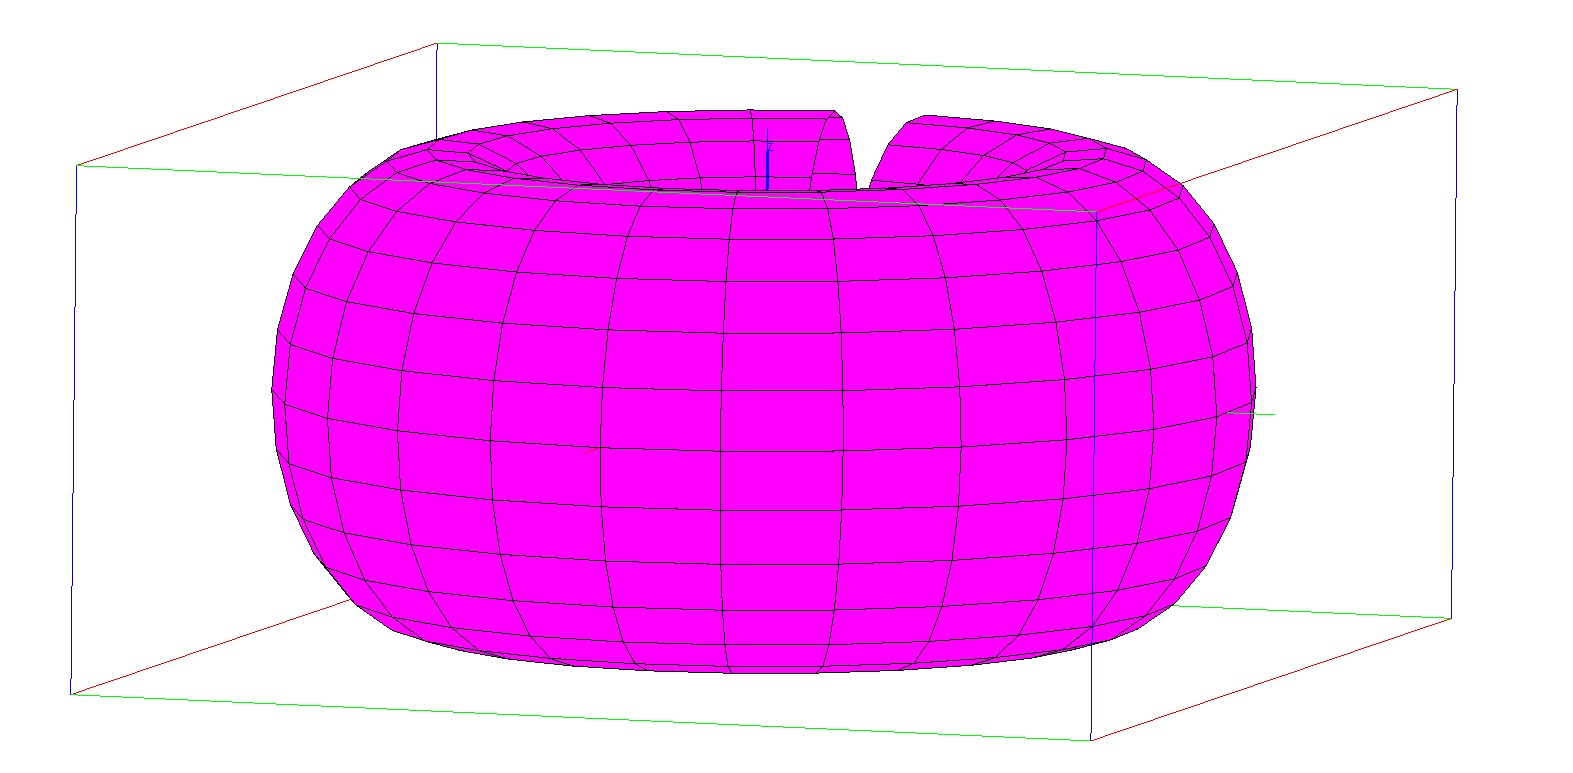
\includegraphics[scale=0.2]{ToreV3}
  \end{center}
\end{enigme}


%%% Local Variables:
%%% mode: latex
%%% TeX-master: "../Manuel-TS"
%%% End:
\end{document}